\documentclass{llncs}

\usepackage{llncsdoc}
\usepackage{graphicx}
\usepackage{float}
\usepackage{algorithmicx}
\usepackage{algorithm}
\usepackage{algpseudocode}
\usepackage{amsmath}
\usepackage{soul}
\usepackage{color}
\usepackage{tikz}
%\usepackage{subfigure}
\usepackage{subfig}




\newcommand{\LD}{\langle}
\newcommand{\RD}{\rangle}




\begin{document}

\title{Verifying Team Formation Protocols in PRISM\thanks{This work is supported by
the ERC Advanced Grant VERIWARE.}}
\author{}
\institute{
  Computing Laboratory, University of Oxford\\
  Wolfson Building, Parks Road, Oxford, OX1 3QD, UK
}
\email{}

\maketitle

\begin{abstract}

Multi-agent systems are becoming an increasingly important paradigm in software. One of the key advantages of multi-agent systems is that agents can cooperate to achieve certain goals, that requires efficient collaboration protocols of which team formation is a typical example. In this paper we illustrate how probabilistic model checking techniques can be applied for analysis, design and verification of such protocols using the PRISM model checker. To start with, we take a simple team formation algorithm and analyse its properties using Discrete-Time Markov Chains, then using Markov Decision Processes we show what is the maximum performance that can be achieved by the protocol which the algorithm uses. And finally we extend the analysis to competitive coalitional setting using Stochastic Two-Player Games.


\end{abstract}

\section{Introduction}

\paragraph{Contributions.}

We point out the advantages of verification by a probabilistic model checker:

\begin{itemize}
  \item easy to compare different organization topology;

  \item easy to compare different strategies, even can \emph{synthesize} the best strategies;

  \item fully-automated

  \item similar to previous scenario from simulation to formal verification

  \item ...
\end{itemize}

\paragraph{Related work.}

Cooperative behaviour being one of the biggest advantages of the agent based computing has been studied from many different angles over the years. Coalitional games traditionally have been analysed from game-theoretic perspective \cite{osborne1994course}, but in recent years has attracted a lot of attention from researchers in artificial intelligence, especially in cooperative task completion \cite{shehory1998methods}. Several approaches for team formation and collaborative task solving are considered including team formation under uncertainty using simple heuristic rules \cite{kraus2003coalition}, reinforcement learning techniques \cite{abdallah2004organization}, and methods using distributed graph algorithms \cite{manisterski2006forming}. To reason formally about cooperative games several several logics  including Coalitional Game Logic \cite{agotnes2009reasoning} and Strategy Logic \cite{chatterjee2007strategy}, and other formalisms one example of which is Cooperative Boolean Games \cite{dunne2008cooperative} have been introduced and used to analyse coalitional behaviours \cite{bonzon2007efficient}. Model checking has been used to analyse a variety of mutli-agent protocol, i.e. clock synchronisation in wireless sensor networks using Uppaal \cite{heidarian2009analysis}, Gossip  \cite{KNP08d} and Byzantine agreement protocols  \cite{KN02} using PRISM   \cite{KNP11}. MCMAS model checker has been applied to verification of knowledge-based properties in multi-agent systems and classic problems like dining cryptographers \cite{lomuscio2006mcmas}.   


Team formation algorithm that we use is introduced in \cite{gaston2005agent}. It has been used for analysis of coalition formation for data fusion in sensor networks \cite{glinton2008agent}.



\paragraph{Structure of the paper.}


\section{Preliminaries}

%% G. Norman and V. Shmatikov.
%Analysis of Probabilistic Contract Signing.
%Journal of Computer Security, 14(6), pages 561-589, IOS Press.


\subsection{Probabilistic Model Checking}

\emph{Probabilistic model checking} is an automated technique for
the formal verification of systems that exhibit stochastic behavior. It can, for example,
calculate the likelihood of the occurrence of certain events
during the execution of a system, and can be useful to establish performance
measures. It is based on the construction and analysis of a
mathematical model of the system, usually from a specification
in some high-level description language. This model
generally comprises a set of states, representing all the possible
configurations of the system, the transitions that can
occur between these states, and information about when and
with what probability each transition will occur, and a probabilistic model checker applies algorithmic techniques to analyze the state space and calculate performance measures.

In this paper, we shall us discrete-time
Markov chains (DTMCs), Markov decision processes (MDPs), and Stochastic Two-Player Games (STPGs) as the modeling formalism. %where time is modelled as
%discrete steps and the probability of making each transition
%is given by a discrete probability distribution.
Below we give a short introduction on these models.

\paragraph{Discrete-Time Markov Chain.}

One of basic models used in probabilistic model checking is \emph{discrete time Markov chains} (DTMCs). A DTMC is defined by a
set of states $S$ and a probability transition matrix
$\mathbf{P} : S\times S \rightarrow [0, 1]$, where
$\sum_{s'\in S} \mathbf{P}(s, s') = 1$ for all $s \in  S$. This gives the probability $\mathbf{P}(s, s')$ that a transition
will take place from state $s$ to state $s'$.


\paragraph{Markov Decision Process}

%M. Duflot, L. Fribourg, T. HšŠrault, R. Lassaigne, F. Magniette, S. Messika, S. Peyronnet and C. Picaronny.
%
%Probabilistic model checking of the CSMA/CD protocol using PRISM and APMC.
Markov Decision Processes (MDP) allow accurate modelling of systems which exhibit
both probabilistic and nondeterministic behavior. Formally, a Markov decision process (MDP) is a tuple $(S, s_0, Act, Steps)$ where $S$ is a finite set of states,
$s_0$ is the initial state, $Act$ is a set of actions
and $Steps\subseteq S \times Act \times Dist(S)$ is a probabilistic transition relation.
An MDP transition $s\stackrel{a,\mu}s'$ is made from a state $s\in S$ first by nondeterministically
selecting an action-distribution pair $(a, \mu)$ such that $(s, a, \mu) \in
steps$, and second by making a probabilistic choice of the target state $s'$ according to the distribution
$\mu$, such that $\mu(s') > 0$. A path represents a particular
%resolution of both nondeterminism and probability: it is a non-empty finite
%or infinite sequence of probabilistic transitions  = s0
%a0,ŠÌ0 ...! s1
%a1,ŠÌ1 ...! ¡€ ¡€ ¡€ such
%that s0 = s. We denote by (i) the (i + 1)-th state of  and last() the
%last state of  if  is finite.

An \emph{adversary} represents a particular resolution
of nondeterminism only. Formally, an adversary of a MDP is a function $A$
mapping every finite path $\pi$ to a pair $(a, \mu)$ such that $(last(\pi), a, \mu)\in Steps$.
The evolution of the MDP according to a particular adversary $A$ is a
measurable set of infinite paths associated with $A$, which can classically be
provided with a probability measure. %Given a set F  S of target states, let:
%P(s A.!
%
%F) denote the probability of reaching F starting from the initial state
%under A.
%The maximal reachability probability Pmax(s ! F), (resp. minimal reach-
%ability probability Pmin(s ! F)), is the maximum (resp. minimum) proba-
%bility over all the adversaries, with which a given set of states can be reached
%from the initial state: Pmax(s ! F) = maxA{P(s A.!
%
%F)} (resp. Pmin(s !
%F) = minA{P(s A.!
%
%F)}).
%Informally, Pmax(s ! F) (resp. Pmin(s ! F)) represents the probability
%that the MDP reaches F, when all non deterministic choices are as favorable
%(resp. unfavorable) as possible.
%Specification of reachability properties to be checked on a MDP may be
%expressed in PCTL, which is a probabilistic extension of the popular temporal
%logic CTL. In [7] the authors provide an algorithm to enrich the usual algo-
%rithm to check a CTL formula on a finite state system, with the computation
%of maximal and minimal probabilities. This can be done in polynomial time
%by solving linear programming systems.


%PRISM [20] is a probabilistic model checker which provides support for
%analysis of Markov decision processes and performs verification of PCTL for-
%mulae for MDPs, using the model checking algorithm of [7]. The most expen-
%sive part of this is the computation of reachability probabilities. For this there
%are two options, either solution of a linear optimization problem or iterative
%numerical solution techniques (based on dynamic programming). PRISM uses
%the second of these. Each iteration computes new values for the reachability
%probabilities, tending towards the exact solution. The computation is ter-
%minated when it has converged to within the desired precision (parameter "
%specified by the user).
%To analyse an MDP, PRISM has to construct the full reachable state space
%and the transition matrix which represents it. However, the tool can often
%handle very large models because it uses symbolic model checking techniques.
%It uses BDD (binary decision diagram) based data structures, in particular
%MTBDDs (multi-terminal BDDs, see e.g. [15]).
%In this paper, we have made use of a prototype extension of PRISM which
%8
%provides support for analysis of properties based on costs (or conversely, re-
%wards) [22]. Each state or transition of the model can be assigned a cost.
%PRISM allows computation of, for example, the expected amount of cost cu-
%mulated before a certain set of states is reached. Because we use MDPs,
%we must compute either the minimum or maximum expected cost (over all
%resolutions of nondeterminism). In PRISM, these properties are expressed as
%(i) Rmin[true Ugoal ]
%(ii) Rmax[true Ugoal ].
%PRISM uses the algorithms of [3] to perform model checking of these for-
%mulas.

\paragraph{Stochastic Two-Player Game}

\paragraph{PCTL}

\subsection{PRISM model checker}

We use PRISM. The current implementation of PRISM supports the analysis of finite state
probabilistic models of the following three types: discrete-time Markov chains,
continuous-time Markov chains and Markov decision processes. These models are
described in a high-level language, a variant of reactive modules [2] based on guarded
commands. The basic components of the language are modules and variables. A
system is constructed as a number of modules which can interact with each other.
A module contains a number of variables which express the state of the module,
and its behavior is given by a set of guarded commands of the form:

[] $\langle$guard$>$ \! $\langle$command$>$;

The guard is a predicate over the variables of the system and the command describes
a transition which the module can make if the guard is true (using primed variables
to denote the next values of variables). If a transition is probabilistic, then the
command is specified as:

$\langle prob \rangle$ : $\langle$ command $\rangle$ + ...+ $\langle$ prob$\rangle$ : <command>

PRISM accepts specifications in either PCTL, or CSL logic depending on the model
type. The model checker then analyses the model and checks if the property holds in each
state.
The reader is invited to consult the PRISM
web site \cite{} for detailed information and corresponding
publications about all of these.

 We use the probabilistic model checking
tool PRISM.% [12, 23]. This allows construction of models
%via specification in a high-level description language, based
%on the parallel composition of several modules described in
%a guarded command notation. We will illustrate the workings
%of this language in more detail later in the paper.
%Models constructed in PRISM are analysed by formally
%specifying formulas in temporal logic. This allows a precise,
%unambiguous description of a wide range of properties, such
%as ¡°the probability of shutdown occurring within 24 hours¡±
%or ¡°the long-run probability that the system is stable¡±. In
%addition, by assigning real-valued costs (or, conversely, rewards)
%to states and transitions of the model, we can also reason
%about, for example, ¡°expected time¡± or ¡°expected power
%consumption¡±.
%PRISM automatically ascertains values for such properties
%by performing probabilistic model checking, which includes
%both graph-based analysis and numerical computation.
%For the case of DTMCs, the latter usually constitutes
%solving a linear equation system of size equal to the number
%of states in the model. For this, PRISM uses iterative numerical
%solution techniques such as the Gauss-Seidel method,
%which are well suited to large problems of this type.
%Furthermore, a significant amount of work has gone into
%the development of efficient, symbolic implementation techniques
%for numerical computation in PRISM. These use data
%structures such as binary decision diagrams (BDDs) [5] and
%their extensions, e.g. multi-terminal BDDs (MTBDDs) [6,
%1], to allow compact storage and manipulation of extremely
%large models. We rely heavily on this efficiency for the case
%study presented in this paper.
%The PRISM tool has already been successfully used to
%perform analysis of, and identify interesting behaviour, in a
%wide range of case studies. This includes the study of ¡°quality
%of service¡± properties for components of real-time probabilistic
%communication protocols, e.g. IEEE 1394 FireWire
%[7, 16], IEEE 802.3 CSMA/CD [17, 8], Zeroconf [13] and
%IEEE 802.11 wireless LANs [15, 24]. It has also been used to
%verify randomised distributed algorithms for leader election,
%consensus [14], Byzantine agreement [10], self-stabilisation
%and mutual exclusion, and probabilistic security protocols
%for anonymity [27], fair exchange and contract signing [20].
%Finally, PRISM has been applied to analysing the performance
%and reliability of many different types of applications:
%dynamic power management schemes [19], NAND
%multiplexing for nanotechnology [18], computer networks,
%queueing systems, manufacturing processes and embedded
%systems [11].



\section{Protocol Modeling and Verification}

\subsection{Definitions}

\cite{gaston2005agent}
In dynamic team formation, agents term form spontaneously in a completely decentralized manner and the agents' decision making is based solely on local information.

In the model, tasks are generated periodically and globally advertised to the organization. Agents attempt to form terms to accomplish these tasks. The agents in the organization are embedded in a social network that restricts the set of possible agent teams: specifically for an agent to be on the team, the agent must have a social connection (i.e., an edge in the social network) with at least one other agent on the team. Tasks are generic in that they only require that a team of agents with the necessary skills form to accomplish the specific task.

\begin{definition}
An agent \textbf{organisation} is a tuple $O=\langle A, N, R, R_A  \rangle$ where
\noindent
\begin{itemize}
\item $A= \{ a_1,a_2,...,a_n \} $ is a set of agents,
\item $N=\{\{a_i,a_j \}\ :$ ``$a_i$ and $a_j$ are neighbours'' $\}$ is a neighbourhood relation,
\item $R=\{r_1,r_2,\dots,r_k\}$ is a set of resource types,
\item $R_A=\{R_{a_1}, R_{a_2}, \dots, R_{a_n}\}$ is a set of agent resources where $r_j \in R_{a_i} $ $\iff$ ``agent $a_i$ has a resource $r_j$''.
\end{itemize}
\end{definition}

\begin{definition}
A \textbf{task} $T_i=\{r_i\ :\ $``$r_i$ is required by the task $i$''$\}$ is a set of resources that are required to complete it. By $T=\{T_1, T_2,\dots, T_t\}$ we denote a collection of tasks.
\end{definition}

\begin{definition}
A \textbf{team} of agents is denoted by $M_i=\{a_i\ :\ $``$a_i$ is a member of team $i$''$\}$, and the set of all teams is $M=\{M_1, M_2,\dots , M_m\}$. By $\bar{M} = \bigcup_{M_i \in M} M_i$ we denote the set of all agents that are committed to some team. $R_{M_i}=\bigcup_{a \in M_i}R_{a}$ is the set of resources that the team $M_i$ has. The team $M_i$ is said to be able to complete the task $T_j$ iff $T_j \subseteq R_{M_i}$.
\end{definition}

\begin{definition}
Team \textbf{initiation probability} for agent $a$ is the ratio between neighbours that are not committed to any team and total number of neighbours:

\begin{equation}
IP_a = \frac{|\{ a' \in A\ :\ \{a, a'\} \in N \wedge a' \notin \bar{M}  \}|}{|\{ a' \in A\ :\ \{a, a'\} \in N \}|}.
\label{eq:init_prob}
\end{equation}

\end{definition}

\begin{definition}
We define two types of \textbf{reward} for agent $a$. Type $W_1$ rewards agent with 1 point if it is in the team which was able to complete its task after team formation is over or 0 otherwise.Type $W_2$ rewards 1 point to the team which was able to complete its task, and 0 otherwise and the reward is shared equally between team members,

\begin{equation}
W_1(a) = \left\{
  \begin{array}{l l}
    1 & \quad \text{if $\exists M_i . a \in M_i \wedge T_i \subseteq R_{M_i}$,}\\
    0 & \quad \text{otherwise,}\\
  \end{array} \right.
\label{eq:w1agent}
\end{equation}
\begin{equation}
W_2(a) = \left\{
  \begin{array}{l l}
    \frac{1}{|M_i|} & \quad \text{if $\exists M_i . a \in M_i \wedge T_i \subseteq R_{M_i}$,}\\
    0 & \quad \text{otherwise.}\\
  \end{array} \right.
\label{eq:w2agent}
\end{equation}

The rewards of a set of agents $A$ are defined accordingly as the total reward achieved by its members,
\begin{equation}
 W_1(A) = \sum_{a \in A} W_1(a),
\label{eq:w1organisation}
\end{equation}
\begin{equation}
 W_2(A) = \sum_{a \in A} W_2(a).
\label{eq:w2organisation}
\end{equation}

\end{definition}

\subsection{Algorithms}


\begin{algorithm}[H]
\caption{Offline and online versions of the algorithm}
\label{alg:main_process}
\begin{scriptsize}
\begin{algorithmic}
\Procedure{Offline}{$t$} \Comment{$t$ - number of tasks}
  \State $M = \{M_i = \emptyset\ :\ 1\leq i \leq t\}$ \Comment{initialise empty teams}
  \State $T = \{T_i\neq \emptyset\ :\ T_i \subseteq_{random} R,\ 1\leq i \leq t\}$ \Comment{initialise tasks at random}
  \ForAll {$a \in A$ in random order}
    \State \Call{JoinTeam}{$a$, $T$, $M$}
  \EndFor
  \State perform tasks and compute rewards
\EndProcedure
\Statex
\Procedure{Online}{$t$} \Comment{$t$ - number of tasks}
  \State $M = \{M_i = \emptyset\ :\ 1\leq i \leq t\}$ \Comment{initialise empty teams}
  \ForAll {$a \in A$ in random order}
    \State \Call{JoinTeam}{$a$, $T$, $M$}
  \EndFor
  \State $T = \{T_i\neq \emptyset\ :\ T_i \subseteq_{random} R,\ 1\leq i \leq t\}$ \Comment{initialise tasks at random}
  \State perform tasks and compute rewards
\EndProcedure

\end{algorithmic}
\end{scriptsize}
\end{algorithm}

\begin{algorithm}[H]
\caption{Team joining algorithm (probabilistic and deterministic)}
\label{alg:join_team_org}
\begin{scriptsize}
\begin{algorithmic}
\Procedure{JoinTeam}{$a$, $T$, $M$}
  \ForAll {$T_i \in T$ in random order}
    \If {$a \notin \bar{M}$} \Comment{agent is not committed}
      \If {$|M_i|=0$} \Comment{team for task i is empty}
	\If {$R_a \cap T_i \neq \emptyset$} \Comment{agent has skill}
	  \State with probability $IP_a$: $M_i \leftarrow M_i \cup \{a\}$ \Comment{initiate a team}
	\EndIf
      \ElsIf {$\exists \{a,a'\} \in N . a' \in M_i$} \Comment{there is neighbour in team for task i}
	\If {$R_a \cap T_i \setminus R_{M_i} \neq \emptyset$} \Comment{agent has a missing resource}
	  \State $M_i \leftarrow M_i \cup \{a\}$ \Comment{join team}
	\EndIf
      \EndIf
    \EndIf
  \EndFor
\EndProcedure
\end{algorithmic}
\end{scriptsize}
\end{algorithm}

\begin{algorithm}[H]
\caption{Team joining algorithm (non-deterministic)}
\label{alg:join_team_nondet}
\begin{scriptsize}
\begin{algorithmic}
\Procedure{JoinTeam}{$a$, $T$, $M$}
  \ForAll {$T_i \in T$ in \hl{arbitrary} order}
    \If {$a \notin \bar{M}$} \Comment{agent is not committed}
      \If {$|M_i|=0$} \Comment{team for task i is empty}
	\If {$R_a \cap T_i \neq \emptyset$} \Comment{agent has skill}
	    \State \hl{$M_i \leftarrow M_i \cup \{a\}$  \textbf{or} $M_i \leftarrow M_i$} \Comment{initiate a team or do nothing}
	\EndIf
      \ElsIf {$\exists \{a,a'\} \in N . a' \in M_i$} \Comment{there is neighbour in team for task i}
	\If {$R_a \cap T_i \setminus R_{M_i} \neq \emptyset$} \Comment{agent has a missing resource}
	  \State \hl{$M_i \leftarrow M_i \cup \{a\}$ \textbf{or} $M_i \leftarrow M_i$} \Comment{join a team or do nothing}
	\EndIf
      \EndIf
    \EndIf
  \EndFor
\EndProcedure
\end{algorithmic}
\end{scriptsize}
\end{algorithm}

\subsection{Experimental Setup}

For our experiments we fix four agent organisations having different properties and then explore team formation algorithms using three models: DTMC, MDP, and STPG. For algorithm \ref{alg:join_team_org} DTMC is the natural model as agents' behaviour is either deterministic or probabilistic, then we relax probabilistic constraints and introduce nondeterminism in algorithm \ref{alg:join_team_nondet}, and to analyse it we use MDP and STPG models. Performance of the algorithms for agent organisations is evaluated from three standpoints:
\begin{enumerate}
 \item Expected overall organisation rewards using equations \ref{eq:w1organisation} and \ref{eq:w2organisation}.
 \item Expected individual agent rewards using equations \ref{eq:w1agent} and \ref{eq:w2agent}.
 \item Expected rewards of agent coalitions using equations \ref{eq:w1organisation} and \ref{eq:w2organisation}.
\end{enumerate}


Online and offline versions described in algorithm \ref{alg:main_process} are equivalent for DTMC (algorithm \ref{alg:join_team_org}) with respect to the evaluation criteria above, but for MDP and STPG (algorithm \ref{alg:join_team_nondet}) we analyse and compare performances of both online and offline algorithms.


\subsubsection{Agent Organisations.}
We run experiments with a set of five agents $A= \{ a_1,a_2,a_3,a_4,a_5 \} $ and a set of  three resources $R=\{r_1,r_2,r_3\}$ arranged in four different agent organisations (see figure \ref{fig:network_configurations} for graphical representations of the organisations):
\begin{itemize}
 \item Fully connected (figure \ref{subfig:fully_connected}) $O_{fc}=\langle A, N_{fc}, R, R_{A_{fc}}  \rangle$ where
    \begin{itemize}
    \item $N_{fc}=\{\{a_i,a_j \}\ : 1 \le i,j \le 5, i\neq j \}$,
    \item $R_{A_{fc}}=\{R_{a_1}, R_{a_2}, R_{a_3}, R_{a_4}, R_{a_5}\}$ where $R_{a_1}=\{r_1\}$, $R_{a_2}=\{r_1\}$, $R_{a_3}=\{r_2\}$, $R_{a_4}=\{r_2\}$, and $R_{a_5}=\{r_3\}$.
    \end{itemize}
 \item Ring (figure \ref{subfig:ring}) $O_r=\langle A, N_r, R, R_{A_r}  \rangle$ where
    \begin{itemize}
    \item $N_r=\{\{a_i,a_j \}\ : 1 \le i,j \le 5, i\neq j, i\le 5 \implies j=i+1, i=5 \implies j=1 \}$,
    \item $R_{A_r}=\{R_{a_1}, R_{a_2}, R_{a_3}, R_{a_4}, R_{a_5}\}$ where $R_{a_1}=\{r_1\}$, $R_{a_2}=\{r_2\}$, $R_{a_3}=\{r_1\}$, $R_{a_4}=\{r_2\}$, and $R_{a_5}=\{r_3\}$.
    \end{itemize}
 \item Star (figure \ref{subfig:star}) $O_s=\langle A, N_s, R, R_{A_s}  \rangle$ where
    \begin{itemize}
    \item $N_s=\{\{a_i,a_j \}\ : 1 \le i,j \le 5, i\neq j, i=1 \}$,
    \item $R_{A_s}=\{R_{a_1}, R_{a_2}, R_{a_3}, R_{a_4}, R_{a_5}\}$ where $R_{a_1}=\{r_1\}$, $R_{a_2}=\{r_2\}$, $R_{a_3}=\{r_2\}$, $R_{a_4}=\{r_3\}$, and $R_{a_5}=\{r_3\}$.
    \end{itemize}
 \item Isolated agent (figure \ref{subfig:isolated}) $O_{ia}=\langle A, N_{ia}, R, R_{A_{ia}}  \rangle$ where
    \begin{itemize}
    \item $N_{ia}=\{\{a_i,a_j \}\ : 1 \le i,j \le 5, i\neq j, (i=5 \vee j=5) \implies (i=4 \vee j=4) \}$,
    \item $R_{A_{ia}}=\{R_{a_1}, R_{a_2}, R_{a_3}, R_{a_4}, R_{a_5}\}$ where $R_{a_1}=\{r_1\}$, $R_{a_2}=\{r_2\}$, $R_{a_3}=\{r_3\}$, $R_{a_4}=\{r_3\}$, and $R_{a_5}=\{r_2\}$.
    \end{itemize}
\end{itemize}
For simplicity we assign one resource to each agent. Resource allocation for each of the agent organisations has been chosen such than it is optimal with respect rewards in equations \ref{eq:w1organisation} and \ref{eq:w2organisation} for algorithm \ref{alg:join_team_org}. Allocations were computed using DTMC model checking in PRISM (see section \ref{subsection:DTMC} for discussion) assuming the task distribution described below.

\subsubsection{Tasks.} We fix seven different tasks that will be used in experiments $T=\{\{r_1\},\{r_2\},\{r_3\},\{r_1,r_2\},\{r_1,r_3\},\{r_2,r_3\},\{r_1,r_2,r_3\}\}$. When running the algorithm two tasks $T_1$ and $T_2$ are picked uniformly and independently at random (with replacement) and are advertised to the agent organisation. So there are total of 49 different combinations of $T_1$ and $T_2$ that can be generated.


\begin{figure}[H]
\centering
\subfloat[Fully connected]{
  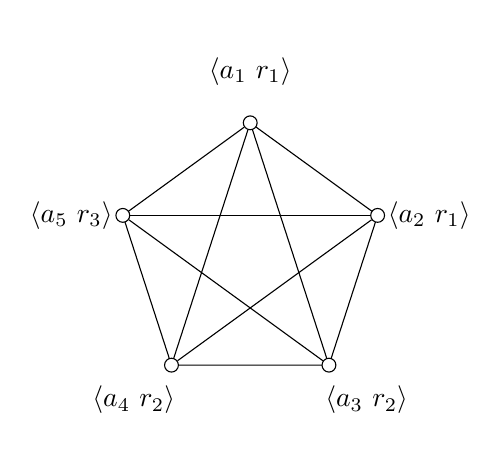
\begin{tikzpicture}
      \tikzstyle{every node}=[draw,circle,fill=white,minimum size=5pt,
			      inner sep=0pt]
      \draw (0,0) 	 node (agent1) [label=90:$\LD a_1\ r_1 \RD$] {}
	  -- ++(-36:2.0cm)   node (agent2) [label=right:$\LD a_2\ r_1 \RD$] {}
	  -- ++(-108:2.0cm) node (agent3) [label=-30:$\LD a_3\ r_2 \RD$] {}
	  -- ++(-180:2.0cm) node (agent4) [label=210:$\LD a_4\ r_2 \RD$] {}
	  -- ++(108:2.0cm) node (agent5) [label=left:$\LD a_5\ r_3 \RD$] {}
	  -- (agent1);
      \draw (agent1) -- (agent3);
      \draw (agent1) -- (agent4);
      \draw (agent2) -- (agent4);
      \draw (agent2) -- (agent5);
      \draw (agent3) -- (agent5);
  \end{tikzpicture}
  \label{subfig:fully_connected}
}\ \ \
\subfloat[Ring]{
  \begin{tikzpicture}
      \tikzstyle{every node}=[draw,circle,fill=white,minimum size=5pt,
			      inner sep=0pt]
      \draw (0,0) 	 node (agent1) [label=90:$\LD a_1\ r_1 \RD$] {}
	  -- ++(-36:2.0cm)   node (agent2) [label=right:$\LD a_2\ r_2 \RD$] {}
	  -- ++(-108:2.0cm) node (agent3) [label=-30:$\LD a_3\ r_1 \RD$] {}
	  -- ++(-180:2.0cm) node (agent4) [label=210:$\LD a_4\ r_2 \RD$] {}
	  -- ++(108:2.0cm) node (agent5) [label=left:$\LD a_5\ r_3 \RD$] {}
	  -- (agent1);
  \end{tikzpicture}
  \label{subfig:ring}
}

\subfloat[Star]{
  \begin{tikzpicture}
      \tikzstyle{every node}=[draw,circle,fill=white,minimum size=5pt,
			      inner sep=0pt]
      \draw (0,0) 	 node (agent1) [label=90:$\LD a_1\ r_1 \RD$] {}
	  -- ++(-36:2.0cm)   node (agent2) [label=right:$\LD a_2\ r_2 \RD$] {}
	   ++(-108:2.0cm) node (agent3) [label=-30:$\LD a_3\ r_2 \RD$] {}
	   ++(-180:2.0cm) node (agent4) [label=210:$\LD a_4\ r_3 \RD$] {}
	   ++(108:2.0cm) node (agent5) [label=left:$\LD a_5\ r_3 \RD$] {}
	  -- (agent1);
      \draw (agent1) -- (agent3);
      \draw (agent1) -- (agent4);
  \end{tikzpicture}
  \label{subfig:star}
}\ \ \
\subfloat[Isolated]{
  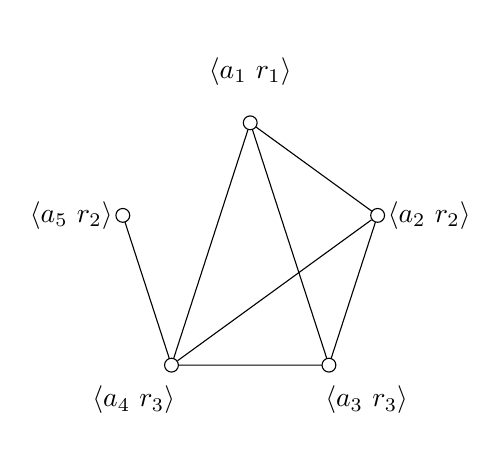
\begin{tikzpicture}
      \tikzstyle{every node}=[draw,circle,fill=white,minimum size=5pt,
			      inner sep=0pt]
      \draw (0,0) 	 node (agent1) [label=90:$\LD a_1\ r_1 \RD$] {}
	  -- ++(-36:2.0cm)   node (agent2) [label=right:$\LD a_2\ r_2 \RD$] {}
	  -- ++(-108:2.0cm) node (agent3) [label=-30:$\LD a_3\ r_3 \RD$] {}
	  -- ++(-180:2.0cm) node (agent4) [label=210:$\LD a_4\ r_3 \RD$] {}
	  -- ++(108:2.0cm) node (agent5) [label=left:$\LD a_5\ r_2 \RD$] {};
      \draw (agent1) -- (agent3);
      \draw (agent1) -- (agent4);
      \draw (agent2) -- (agent4);
  \end{tikzpicture}
  \label{subfig:isolated}
}

\caption{Experimental configurations of the agent organisations with optimal resource allocation (see table \ref{tab:optimal_r}).}
\label{fig:network_configurations}
\end{figure}



\subsection{DTMC}
\label{subsection:DTMC}
\subsubsection{Protocol}
\subsubsection{Model and Specification}
\subsubsection{Results}


\begin{table}
 \centering
 \begin{tabular}{ | l | l | l | l |}
    \hline
    Agents & States & Transitions & Construction Time \\ \hline
    2 & 1865 & 2256 & 0.112s  \\ \hline
    3 & 17041 & 20904 & 0.311s \\ \hline
    4 & 184753 & 226736 & 3.347s \\ \hline
    5 & 2366305 & 2893536 & 74.36s \\ \hline
    6 & 35058241 & 42638400 & 2916.235s \\ \hline
\end{tabular}
\caption{DTMC model comparison for different number of agents in fully connected agent organisation. Model construction times are for 2.8GHz, 4Gb RAM PC.}
\end{table}

\begin{table}
 \centering
 \begin{tabular}{ | l | l | l | l |}
    \hline
    Organisation $O$ & Additional constraints & Example $\LD R_{a_1}R_{a_2}R_{a_3}R_{a_4}R_{a_5}\RD$ \\ \hline
    $O_{fc}$ & - & $R_A=\LD \{r_1\}\{r_1\}\{r_2\}\{r_2\}\{r_3\}\RD$  \\ \hline
    $O_r$ & $R_{a_1}\neq R_{a_5} \wedge \forall i < 5 . R_{a_i} \neq  R_{a_{i+1}} $ & $R_A=\LD \{r_1\}\{r_2\}\{r_1\}\{r_2\}\{r_3\}\RD$  \\ \hline
    $O_s$ & $R_{a_1}=\{r\} \wedge \forall i > 1 . r \notin R_{a_i} $  & $R_A=\LD \{r_1\}\{r_2\}\{r_2\}\{r_3\}\{r_3\}\RD$  \\ \hline
    $O_{ia}$ & $R_{a_5}=\{r\} \wedge \exists i < 4 . r \in R_{a_i} $ & $R_A=\LD \{r_1\}\{r_2\}\{r_3\}\{r_3\}\{r_2\}\RD$  \\ \hline
\end{tabular}
\caption{Optimal resource allocations ($R_A$) for agent organisations from figure \ref{fig:network_configurations} with respect to rewards defined in equations \ref{eq:w1organisation} and \ref{eq:w2organisation}. All allocations satisfy the following constraint $\forall i. |R_{a_i}|=1 \wedge   \forall i.1 \le|\{ R_{a_j} : r_i \in R_{a_j} (1 \le j \le 5 )\}|\le 2$. That is each agent is allocated exactly one resource, each resource is allocated to some agent, no resource is allocated to more than 2 agents}
\label{tab:optimal_r}
\end{table}


\begin{table}
\subfloat[Using $W_1$ reward structure.]{
%\begin{table}
% \centering
 \begin{tabular}{ | l | l | l | l | l |}
    \hline
    $O$ & $W_1(O)$ & $\min_{a \in A}W_1(a)$ & $\max_{a \in A}W_1(a)$ \\ \hline
    $O_{fc}$ & 2.54906 & 0.44958 & 0.75073   \\ \hline
    $O_r$  & 2.30359 & 0.35494 & 0.63985 \\ \hline
    $O_s$  & 1.87278 & 0.28677 & 0.72568  \\ \hline
    $O_{ia}$  & 2.38529 & 0.28867 & 0.68769  \\ \hline
\end{tabular}
%\caption{Model checking results for reward $W_1$.}
%\end{table}
}
\subfloat[Using $W_2$ reward structure.]{
%\begin{table}
% \centering
 \begin{tabular}{ | l | l | l | l |}
    \hline
    $O$ & $W_2(O)$ & $\min_{a \in A}W_2(a)$ & $\max_{a \in A}W_2(a)$ \\ \hline
    $O_{fc}$ & 1.49125 & 0.26721 & 0.42238 \\ \hline
    $O_r$ & 1.42923 & 0.23531 & 0.38625 \\ \hline
    $O_s$ & 1.16649 & 0.18582 & 0.42321  \\ \hline
    $O_{ia}$ & 1.43599 & 0.20621 & 0.39907  \\ \hline
\end{tabular}
%\caption{Model checking results for reward $W_2$.}
%\end{table}
}
\caption{Model checking results for agent organisations from figure \ref{fig:network_configurations} with optimal resource allocations from table \ref{tab:optimal_r}. Tables also show largest and smallest individual agent rewards. }
\end{table}


\begin{table}
 \centering
 \begin{tabular}{ | l | l | l | l |}
    \hline
    Organisation & $T_1$ completed & $T_2$ completed & $T_1$ and $T_2$ completed \\ \hline
    $O_{fc}$ & 0.74562 & 0.74562 & 0.49596  \\ \hline
    $O_r$ & 0.71461 & 0.71461 & 0.47062 \\ \hline
    $O_s$ & 0.58324 & 0.58324 & 0.23639 \\ \hline
    $O_{ia}$ & 0.71799 & 0.71799 & 0.44839 \\ \hline
\end{tabular}

\caption{Task completion probabilities for optimal agent organisations using algorithm \ref{alg:join_team_org}. Results obtained by model checking PCTL formulae on DTMC model.}
\end{table}

\clearpage

\subsection{MDP}
\subsubsection{Protocol}
\subsubsection{Model and Specification}
\subsubsection{Results}
\begin{table}
 \centering
 \begin{tabular}{ | l | l | l | l |}
    \hline
    Agents & States & Transitions & Construction Time \\ \hline
    2 & 1405 & 1846 & 0.045s  \\ \hline
    3 & 9721 & 12474 & 0.167s \\ \hline
    4 & 76865 & 96664 & 1.109s \\ \hline
    5 & 731233 & 907992 & 5.0536s \\ \hline
    6 & 8155873 & 10040112 & 29.74s \\ \hline
\end{tabular}
\caption{MDP model comparison for different number of agents in fully connected agent organisation. Model construction times are for 2.8GHz, 4Gb RAM PC.}
\end{table}

\begin{table}
\centering
\subfloat[Offline]{
 \begin{tabular}{ | l | l | l | l |}
    \hline
    $O$ & Max $W_1(O)$ & Max $W_2(O)$ \\ \hline
    $O_{fc}$ & 2.89795 & 1.67346   \\ \hline
    $O_r$ & 2.89795 & 1.67346  \\ \hline
    $O_s$ & 2.20816 & 1.35918  \\ \hline
    $O_{ia}$ & 2.89795 & 1.67346  \\ \hline
\end{tabular}
}
\subfloat[Online]{
 \begin{tabular}{ | l | l | l | l |}
    \hline
    $O$ & Max $W_1(O)$ & Max $W_2(O)$ \\ \hline
    $O_{fc}$ & 3.85714 & 1.42857   \\ \hline
    $O_r$ & 3.85714 & 1.42857  \\ \hline
    $O_s$ & 2.71428 & 1.02857  \\ \hline
    $O_{ia}$ & 3.85714 & 1.42857  \\ \hline
\end{tabular}
}
\caption{Maximal rewards that can be achieved by agent organisations from figure \ref{fig:network_configurations} using algorithm \ref{alg:join_team_nondet}'s offline and online versions defined in algorithm \ref{alg:main_process}.}
\end{table}


\begin{table}

 \centering

\subfloat[Offline]{
 \begin{tabular}{ | l | l | l | l |}
    \hline
    $O$ & $T_1$ compl. & $T_2$ compl. & $T_1$ and $T_2$ compl. \\ \hline
    $O_{fc}$ & 1.0 & 1.0 & 0.67346  \\ \hline
    $O_r$ & 1.0 & 1.0 & 0.67346  \\ \hline
    $O_s$ & 0.82857 & 0.82857 & 0.39183 \\ \hline
    $O_{ia}$ & 1.0 & 1.0 & 0.67346 \\ \hline
\end{tabular}
}
\subfloat[Online]{
 \begin{tabular}{ | l | l | l | l |}
    \hline
    $O$ & $T_1$ compl. & $T_2$ compl. & $T_1$ and $T_2$ compl. \\ \hline
    $O_{fc}$ & 1.0 & 1.0 & 0.42857  \\ \hline
    $O_r$ & 1.0 & 1.0 & 0.42857 \\ \hline
    $O_s$ & 0.88571 & 0.88571 & 0.12653 \\ \hline
    $O_{ia}$ & 1.0 & 1.0 & 0.42857 \\ \hline
\end{tabular}
}

\caption{Maximum task completion probabilities for optimal agent organisations using algorithm \ref{alg:join_team_nondet}'s online and offline versions (see algorithm \ref{alg:main_process}). Results obtained by model checking PCTL formulae on MDP model.}
\end{table}

\clearpage

\subsection{STPG}
\subsubsection{Protocol}
\subsubsection{Model and Specification}
\subsubsection{Results}

\begin{table}
 \centering
 \begin{tabular}{ | l | l | l | l | l | l |}
    \hline
    $O$ & 1& 2 & 3 & 4 & 5 \\ \hline
    $O_{fc}$ & $\LD r_1 \RD$ & $\LD r_1, r_2 \RD$ & $\LD r_1, r_2, r_4 \RD$ & $\LD r_1, r_2, r_3, r_4 \RD$  & $\LD r_1, r_2, r_3, r_4, r_5 \RD$ \\ \hline
    $O_r$ & $\LD r_1 \RD$  & $\LD r_2, r_3 \RD$ & $\LD r_1, r_4, r_5 \RD$ & $\LD r_1, r_2, r_4, r_5 \RD$  & $\LD r_1, r_2, r_3, r_4, r_5 \RD$\\ \hline
    $O_s$ & $\LD r_1 \RD$  & $\LD r_1, r_2 \RD$ & $\LD r_1, r_2, r_4 \RD$ & $\LD r_1, r_2, r_3, r_4 \RD$  & $\LD r_1, r_2, r_3, r_4, r_5 \RD$\\ \hline
    $O_{ia}$ & $\LD r_1 \RD$  & $\LD r_1, r_4 \RD$ & $\LD r_1, r_2, r_4 \RD$ & $\LD r_1, r_2, r_4, r_5 \RD$  & $\LD r_1, r_2, r_3, r_4, r_5 \RD$\\ \hline
\end{tabular}
\caption{Optimal coalitions of sizes 2, 3, and 4 for agent organisations from figure \ref{fig:network_configurations} for both online and offline versions.}
\label{tab:optimal_coalitions}
\end{table}

\begin{table}
 \centering
\subfloat[Offline]{
  \begin{tabular}{ | l | l | l | l | l | l |}
      \hline
      $O$ & 1 & 2 & 3 & 4 & 5 \\ \hline
      $O_{fc}$ & 0.14285 & 0.42857 & 1.0 & 1.0 & 1.0  \\ \hline
      $O_r$ & 0.14285 & 0.42857 & 0.68333 &  0.92619 & 1.0 \\ \hline
      $O_s$ & 0.14285 & 0.42857 & 0.79761 & 0.81904 & 0.82857\\ \hline
      $O_{ia}$ & 0.14285 & 0.42857 & 0.93452 & 1.0 & 1.0\\ \hline
  \end{tabular}
}
\subfloat[Online]{
  \begin{tabular}{ | l | l | l | l | l | l |}
      \hline
      $O$ & 1 & 2 & 3 & 4 & 5 \\ \hline
      $O_{fc}$ & 0.14285 & 0.42857 & 1.0 & 1.0 & 1.0  \\ \hline
      $O_r$ & 0.14285 & 0.33333 & 0.68571 & 0.89523 & 1.0 \\ \hline
      $O_s$ & 0.14285 & 0.42857 & 0.76190 & 0.84761 & 0.88571 \\ \hline
      $O_{ia}$ & 0.14285 & 0.42857 & 0.92857 & 1.0 & 1.0\\ \hline
  \end{tabular}
}
\caption{Values for maximum probabilities to complete one task for coalitions from table \ref{tab:optimal_coalitions}.}
\end{table}


\begin{table}
 \centering
\subfloat[Offline]{
 \begin{tabular}{ | l | l | l | l | l | l |}
    \hline
    $O$ & 1 & 2 & 3 & 4 & 5 \\ \hline
    $O_{fc}$ & 0.0 & 0.04081 & 0.24489 &  0.42857 & 0.67346  \\ \hline
    $O_r$ & 0.0 &  0.04081 & 0.17687 & 0.40748 & 0.67346\\ \hline
    $O_s$ & 0.0 & 0.04081 & 0.20408 & 0.29523 & 0.39183 \\ \hline
    $O_{ia}$ & 0.0 & 0.04081 & 0.23129 & 0.41496 & 0.67346\\ \hline
\end{tabular}
}
\subfloat[Online]{
 \begin{tabular}{ | l | l | l | l | l | l |}
    \hline
    $O$ & 1 & 2 & 3 & 4 & 5 \\ \hline
    $O_{fc}$ & 0.0 & 0.02040 & 0.06122 &  0.18367 & 0.42857  \\ \hline
    $O_r$ & 0.0 & 0.02040 & 0.06122 & 0.18367 & 0.42857\\ \hline
    $O_s$ & 0.0 & 0.02040 & 0.06122 & 0.12244 & 0.12653 \\ \hline
    $O_{ia}$ & 0.0 & 0.02040 & 0.06122 & 0.18231 & 0.42857\\ \hline
\end{tabular}
}

\caption{Values for maximum probabilities to complete both tasks for coalitions from table \ref{tab:optimal_coalitions}.}
\end{table}

\section{Conclusions and Future Work}

We would like to outline several directions for future work:
\begin{itemize}

 \item Conducting experiments with agents having multiple resources, allowing agents to change teams until stable point is reached and check whether it can reached, what is the expected number of steps to reach the stable configuration, etc.

\item Verifying dual properties, i.e. rather than asking ``what is the expected reward for a strategy'', we would like to be able to model-check the properties of the form ``whats is the probability of reaching reward value R with a strategy?''.

 \item In this paper we only considered sequential execution of agent algorithms, in future work we would like to explore parallel execution (i.e. interleaving steps of JoinTeam algorithm for multiple agents), and see what effect this has for agent strategies in both online and offline versions of the algorithm. Also this raises many interesting scheduling problems, as worst and best case scheduling (of action interleaving) scenarios are unrealistic, the challenging question is to both develop realistic schedulers and perform model-checking efficiently.

 \item Another interesting question is construction of optimal agent organisations given the set of tasks and their distributions.This problem is an instance of mechanism design problem in game-theoretic settings, where the designer can have control over neighbourhood structure or agent resources or both.

\end{itemize}

\bibliographystyle{plain}
\bibliography{refs}

\end{document} 